\documentclass[]{BasiliskReportMemo}
\usepackage{AVS}

\newcommand{\submiterInstitute}{Autonomous Vehicle Simulation (AVS) Laboratory,\\ University of Colorado}

\newcommand{\ModuleName}{thrMomentumManagement}
\newcommand{\subject}{Reaction Wheel Angular Momentum Dumping Management Module}
\newcommand{\status}{Initial Document draft}
\newcommand{\preparer}{H. Schaub}
\newcommand{\summary}{This module reads in the Reaction Wheel (RW) speeds, determines the net RW momentum, and then determines the amount of angular momentum that must be dumped.  A separate thruster firing logic module called {\tt thrMomentumDumping} will later on compute the thruster on cycling.      }


\begin{document}


\makeCover


%
%	enter the revision documentation here
%	to add more lines, copy the table entry and the \hline, and paste after the current entry.
%
\pagestyle{empty}
{\renewcommand{\arraystretch}{1.1}
\noindent
\begin{longtable}{|p{0.5in}|p{4.5in}|p{1.14in}|}
\hline
{\bfseries Rev}: & {\bfseries Change Description} & {\bfseries By} \\
\hline
Draft & Initial document creation & H. Schaub \\
0.1 & Updated the sign of $\leftexp{B}{\Delta\bm H}$ & H. Schaub \\
\hline

\end{longtable}
}

\newpage
\setcounter{page}{1}
\pagestyle{fancy}

\tableofcontents
~\\ \hrule ~\\

\begin{figure}[htb]
	\centerline{
	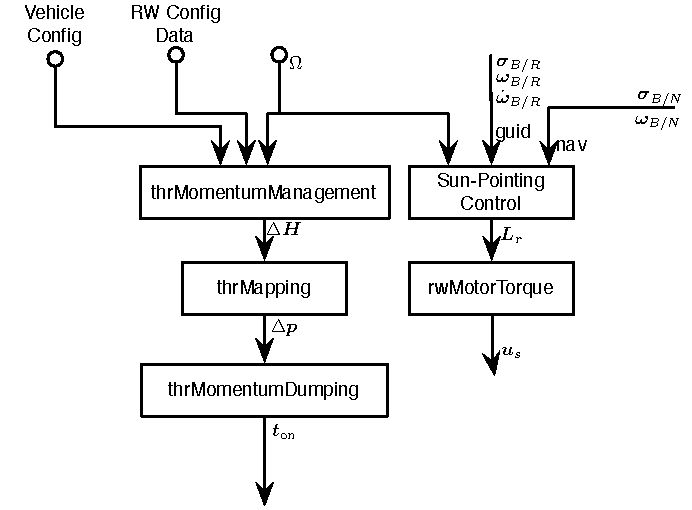
\includegraphics[]{Figures/rwMomentumOverview}
	}
	\caption{Overview of the Modules Used to Perform Reaction Wheel Angular Momentum Dumping.}
	\label{fig:Fig1}
\end{figure}

\section{Introduction}
To manage the Reaction Wheel (RW) angular momentum build-up over time, a thruster-based momentum dumping strategy is used.  Figure~\ref{fig:Fig1} illustrates how the momentum dumping will occur simultaneously with an inertial pointing control solution.  Assume the spacecraft contains $N_{\text{RW}}$ RWs, and $M_{\text{thr}}$ thrusters. The net RW angular momentum is given by
\begin{equation}
	\bm h_{s} = \sum_{i=1}^{N_{\text{RW}}} \hat{\bm g}_{s_{i}} \Omega_{i}
\end{equation} 
where $\hat{\bm g}_{s_{i}}$ is the RW spin axis, and $\Omega_{i}$ is the RW speed rate about this axis.  
Because the inertial attitude of the spacecraft is assumed to be held nominally steady, 
\begin{equation}
	\dot{\bm h}_{s} = \frac{\leftexp{B}{\D}\bm h_{s}}{\D t} + \bm\omega_{B/N} \times \bm h_{s} \approx \frac{\leftexp{B}{\D}\bm h_{s}}{\D t}
\end{equation}






\begin{figure}[tp]
	\centerline{
	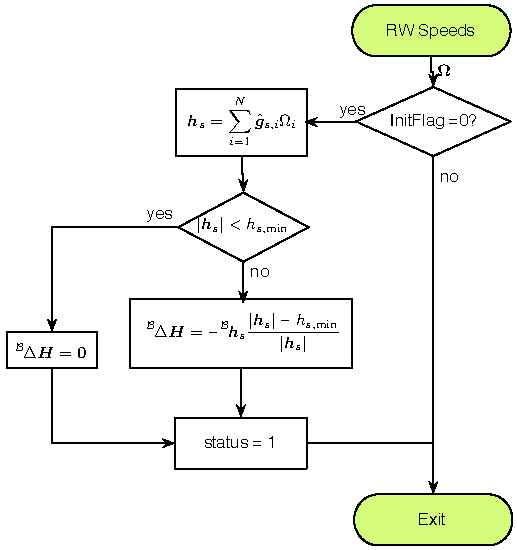
\includegraphics[]{Figures/rwMomentumManagement}
	}
	\caption{Overview of the Reaction Wheel Angular Momentum Management Module.}
	\label{fig:Fig2}
\end{figure}

\section{{\tt thrMomentumManagement}  Module Description}
Figure~\ref{fig:Fig2} illustrates the function of the RW angular momentum dumping management module.  Let $h_{s,\text{min}}$ be lower bound that the RW momentum dumping strategy should achieve.  The desired net change in inertial angular momentum is thus determined through
\begin{equation}
	\leftexp{B}{\Delta}\bm H = -\leftexp{B}{\bm h}_{s} \frac{
		|\bm h_{s}| - h_{s,\text{min}}
	}{|\bm h_{s}|} 
\end{equation}

This strategy requires a thruster firing solution which creates this desired $\leftexp{B}{\Delta}\bm H$ over the duration of the momentum dumping.  The goal of the RW momentum management module is to simply compute if a $\leftexp{B}{\Delta}\bm H$ is required, or set it equal to zero if the RW momentum is too small.  Not that this module will only compute $\leftexp{B}{\Delta}\bm H$ once.  Either it is zero or non-zero.  To reuse this momentum management module, the reset() function must be called.




\section{Module Parameters}
\subsection{{\tt hs\_min} Parameter}
This parameter dictates the desired lower ceiling of the RW cluster angular momentum.  It must be set prior to calling the routine.  



\end{document}
